% Restoration pipeline block diagram (slide version), ECE 253 course conventions:
% light-blue bordered blocks, wide hollow arrows, dashed grouping box, proposal's
% modified block in yellow. Build: tectonic bleed/diagrams/pipeline.tex
\documentclass[border=8pt]{standalone}
\usepackage{amsmath,amssymb,bm}
\usepackage{tikz}
\usetikzlibrary{shapes.arrows,positioning,shadows,fit,calc}

\definecolor{blockedge}{HTML}{7FA7D9}
\definecolor{navy}{HTML}{1F3B73}
\definecolor{hl}{HTML}{FFF2A8}

\tikzset{
  blk/.style={draw=blockedge, line width=0.9pt, fill=white, text width=6.0cm,
              minimum height=3.6cm, align=center, drop shadow={opacity=0.22, shadow xshift=0.6mm, shadow yshift=-0.6mm}},
  harrow/.style={single arrow, draw=black, fill=white, line width=0.6pt, minimum height=1.05cm,
                 single arrow head extend=0.12cm, inner sep=1.6pt},
}
\newcommand{\ttl}[2]{\textcolor{navy}{\bfseries\Large #1}\\\textcolor{navy}{\bfseries\Large #2}}
\newcommand{\hollow}[2]{% hollow block arrow from #1 to #2 (horizontal)
  \path let \p1=(#1), \p2=(#2), \n1={veclen(\x2-\x1,\y2-\y1)} in
    node[harrow, minimum height=\n1, anchor=tail] at (#1) {};}

\begin{document}
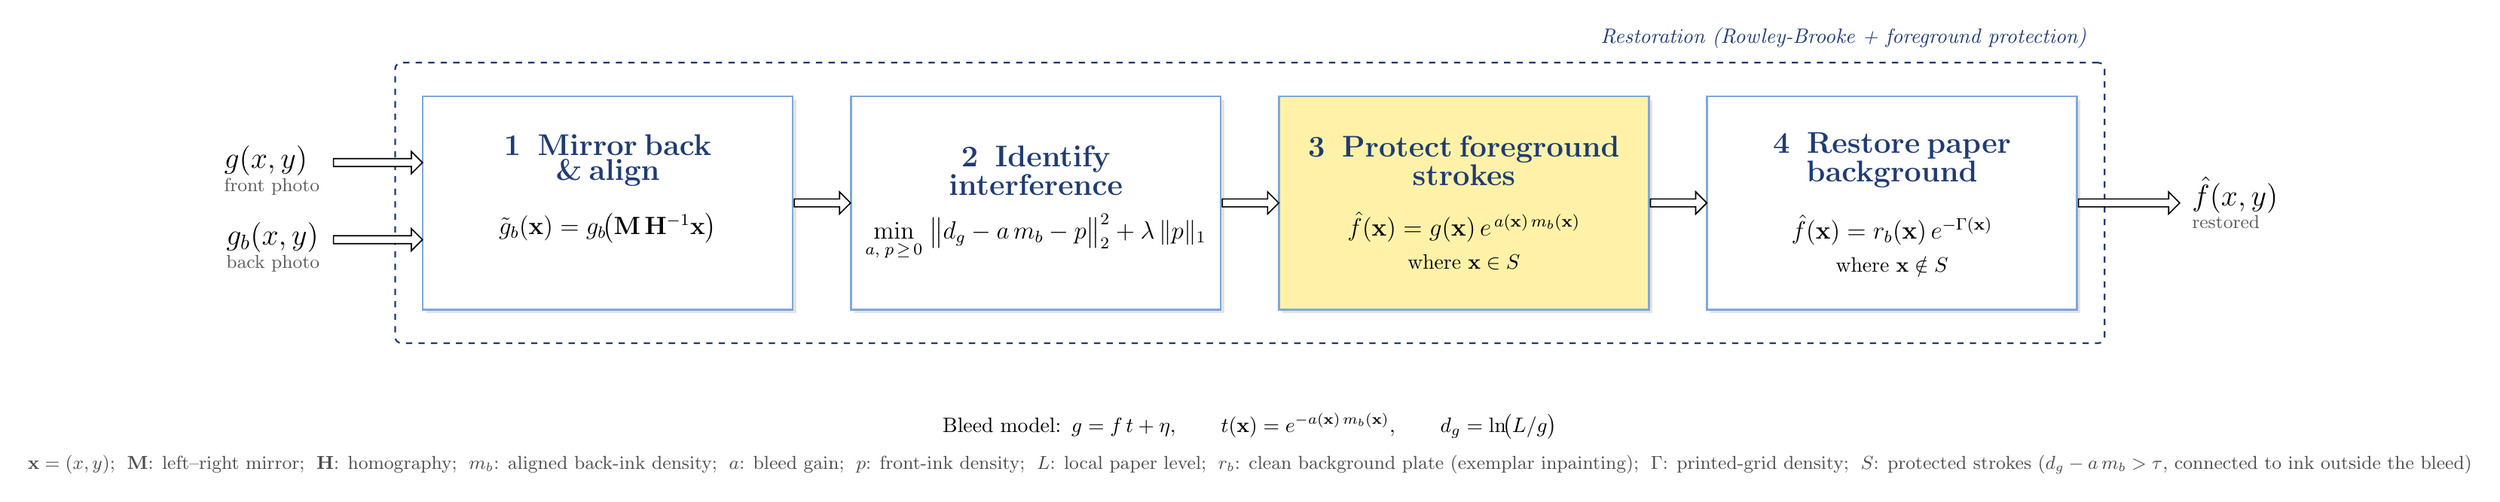
\begin{tikzpicture}[node distance=0.95cm]
  % restoration blocks
  \node[blk] (b1) {\ttl{1\enspace Mirror back}{\& align}\\[12pt]
                   \mbox{\large $\tilde{g}_b(\mathbf{x}) = g_b\!\bigl(\mathbf{M}\,\mathbf{H}^{-1}\mathbf{x}\bigr)$}\\[4pt]\phantom{$p$}};
  \node[blk, right=of b1] (b2) {\ttl{2\enspace Identify}{interference}\\[8pt]
                   \mbox{\large $\displaystyle\min_{a,\;p\,\ge\,0}\;\bigl\lVert d_g - a\,m_b - p\bigr\rVert_2^2 + \lambda\,\lVert p\rVert_1$}};
  \node[blk, right=of b2, fill=hl] (b3) {\ttl{3\enspace Protect foreground}{strokes}\\[12pt]
                   \mbox{\large $\hat{f}(\mathbf{x}) = g(\mathbf{x})\,e^{\,a(\mathbf{x})\,m_b(\mathbf{x})}$}\\[4pt]
                   \mbox{\normalsize where $\mathbf{x}\in S$}};
  \node[blk, right=of b3] (b4) {\ttl{4\enspace Restore paper}{background}\\[12pt]
                   \mbox{\large $\hat{f}(\mathbf{x}) = r_b(\mathbf{x})\,e^{-\Gamma(\mathbf{x})}$}\\[4pt]
                   \mbox{\normalsize where $\mathbf{x}\notin S$}};

  % dashed restoration group
  \node[draw=navy, dashed, line width=0.8pt, rounded corners=3pt, inner xsep=0.45cm, inner ysep=0.55cm,
        fit=(b1)(b2)(b3)(b4)] (grp) {};
  \node[anchor=south east, font=\itshape, text=navy] at ([xshift=-2mm, yshift=1mm]grp.north east)
        {Restoration (Rowley-Brooke + foreground protection)};

  % inputs
  \node[anchor=east, align=left] (g)  at ([xshift=-1.6cm, yshift= 0.55cm]b1.west) {\Large $g(x,y)$\\[-1pt]{\small\color{black!65} front photo}};
  \node[anchor=east, align=left] (gb) at ([xshift=-1.6cm, yshift=-0.75cm]b1.west) {\Large $g_b(x,y)$\\[-1pt]{\small\color{black!65} back photo}};
  \hollow{$(g.east)+(0.1,0.13)$}{$(b1.west|-g.east)+(0,0.13)$}
  \hollow{$(gb.east)+(0.1,0.13)$}{$(b1.west|-gb.east)+(0,0.13)$}

  % chain + output
  \hollow{b1.east}{b2.west}
  \hollow{b2.east}{b3.west}
  \hollow{b3.east}{b4.west}
  \node[anchor=west, align=left] (out) at ([xshift=1.8cm]b4.east) {\Large $\hat{f}(x,y)$\\[-1pt]{\small\color{black!65} restored}};
  \hollow{b4.east}{$(out.west)+(-0.1,0.13)$}

  % model and symbol key
  \node[below=1.05cm of grp.south, align=center] {%
    Bleed model:\enspace $g = f\,t + \eta,\qquad t(\mathbf{x}) = e^{-a(\mathbf{x})\,m_b(\mathbf{x})},\qquad
    d_g = \ln\!\bigl(L/g\bigr)$\\[6pt]
    {\small\color{black!70}$\mathbf{x}=(x,y)$;\; $\mathbf{M}$: left--right mirror;\; $\mathbf{H}$: homography;\;
    $m_b$: aligned back-ink density;\; $a$: bleed gain;\; $p$: front-ink density;\;
    $L$: local paper level;\; $r_b$: clean background plate (exemplar inpainting);\; $\Gamma$: printed-grid density;\; $S$: protected strokes ($d_g-a\,m_b>\tau$, connected to ink outside the bleed)}};
\end{tikzpicture}
\end{document}
